% Diagrama clasico de energia/coenergia magnetica en el plano i-lambda.
% Ilustra, para una posicion x fija, el enlace de flujo lambda(i,x) y como
% la curva reparte el rectangulo i0*lambda0 en dos areas complementarias.
\definecolor{tray}{RGB}{31,94,166}
\definecolor{ctl2}{RGB}{196,96,40}
\definecolor{refc}{RGB}{40,40,40}
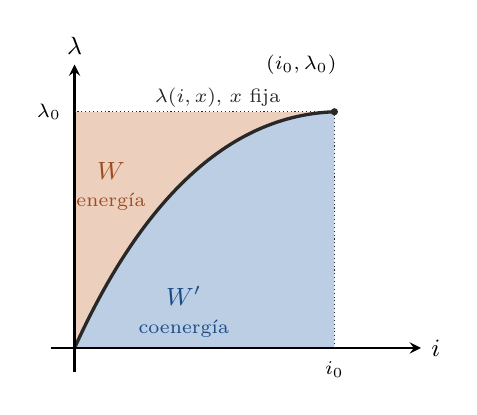
\begin{tikzpicture}[>=stealth, font=\small]
  \def\imax{4.4} \def\lmax{3.6}
  \def\izero{3.3} \def\lzero{3.0}
  % curva lambda(i) a x fija, forma de saturacion
  \pgfmathsetmacro{\curvepath}{0}
  % areas, dibujadas antes que los ejes para que estos queden encima
  \fill[tray!55, opacity=0.55]
    (0,0) .. controls (\izero*0.35,\lzero*0.85) and (\izero*0.75,\lzero*0.99) .. (\izero,\lzero)
    -- (\izero,0) -- cycle;
  \fill[ctl2!55, opacity=0.55]
    (0,0) .. controls (\izero*0.35,\lzero*0.85) and (\izero*0.75,\lzero*0.99) .. (\izero,\lzero)
    -- (0,\lzero) -- cycle;
  % curva encima de las areas
  \draw[very thick, refc] (0,0) .. controls (\izero*0.35,\lzero*0.85) and (\izero*0.75,\lzero*0.99) .. (\izero,\lzero);
  % ejes
  \draw[->, thick] (-0.3,0) -- (\imax,0) node[right] {$i$};
  \draw[->, thick] (0,-0.3) -- (0,\lmax) node[above] {$\lambda$};
  % guias punteadas al punto de operacion
  \draw[densely dotted, refc] (\izero,0) -- (\izero,\lzero) -- (0,\lzero);
  \fill[refc] (\izero,\lzero) circle (1.3pt);
  \node[anchor=south east, font=\scriptsize] at (\izero+0.15,\lzero+0.35) {$(i_0,\lambda_0)$};
  \node[anchor=north, font=\scriptsize] at (\izero,-0.05) {$i_0$};
  \node[anchor=east, font=\scriptsize] at (-0.05,\lzero) {$\lambda_0$};
  % etiquetas de las areas (apiladas, para que no se encimen)
  \node[tray!80!black, font=\small] at (\izero*0.42,\lzero*0.22) {$W'$};
  \node[tray!80!black, font=\scriptsize] at (\izero*0.42,\lzero*0.08) {coenergía};
  \node[ctl2!80!black, font=\small] at (\izero*0.14,\lzero*0.75) {$W$};
  \node[ctl2!80!black, font=\scriptsize] at (\izero*0.14,\lzero*0.62) {energía};
  % curva etiquetada, lejos del punto de operacion para no encimarse
  \node[refc, font=\scriptsize, anchor=south, yshift=4pt] at (\izero*0.55,\lzero*0.93) {$\lambda(i,x)$, $x$ fija};
\end{tikzpicture}
